\onehalfspaced

\section{Estimating Translation Quality}
We use a linear regression model\footnote{We used WEKA package: \url{http://www.cs.waikato.ac.nz/ml/weka/}} to predict a quality score ($ score(t) \in R$) for an input translation $t$.
%\begin{align*}
\[ score(t) = \vec{w}  \cdot \vec f(t) \]
  %\end{align*}
  where $\vec{w}$ is the associated weight vector and $\vec f(t)$ is the feature vector of the translation $t$. 

We replicate the feature set used by \newcite{zaidan-callisonburch:2011:ACL-HLT2011a} in their MERT model:

\begin{itemize}
\item  Sentence-level features: 9 features based on language model, sentence length, edit distance to other translations. 
\item Worker-level features: 15 features based on worker's language ability, location and average sentence-level scores.
\item Ranking features: 3 features based on the judgments of monolingual English speakers ranking the translations from best to worst.
\item Calibration features: 1 feature based on the average BLEU score of translations provided by the same worker, which is computed against professional references.
%\item Bilingual features: 1 feature based on the word alignment probabilities according. 
\end{itemize}


We additionally introduce a new bilingual feature based on IBM Model 1. We align words between each candidate translation and its corresponding source sentence. The bilingual feature for a translation is the average of its alignment probabilities. In Figure \ref{biexample1}, we show how the bilingual feature allows us to distinguish between a valid translation (top) and an invalid/spammy translation (bottom).

\begin{figure}
  \centering
  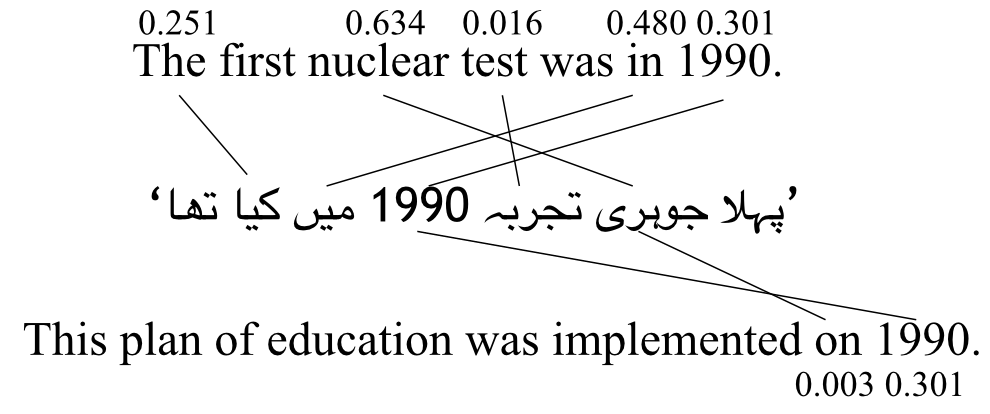
\includegraphics[width=\linewidth]{bilingualexample/example.png}
  \caption{Example bilingual feature for two crowdsourced translations for a sentence in Urdu. The numbers are alignment probabilities for each aligned word. The bilingual feature is the average of these probabilities, thus 0.240 for the good translation and 0.043 for the bad translation. Some words are not aligned if potential word pairs don't exist in corpus.
}
    \label{biexample1}
\end{figure}

%\newcite{zaidan-callisonburch:2011:ACL-HLT2011a} used all 4 professional translations in computing the calibration features and training labels. We will show in the experiments that using \textbf{only one} professional translation as reference is as sufficient. 
